% PGFPlots Basics
% Demonstrates: function plots, scatter plots, bar charts, and axis customization.
% Compile with: pdflatex main.tex
% Requires: pgfplots package (included in most TeX distributions)

\documentclass{article}
\usepackage{pgfplots}
\pgfplotsset{compat=1.18}

\begin{document}

% --- Line plot: sin and cos ---
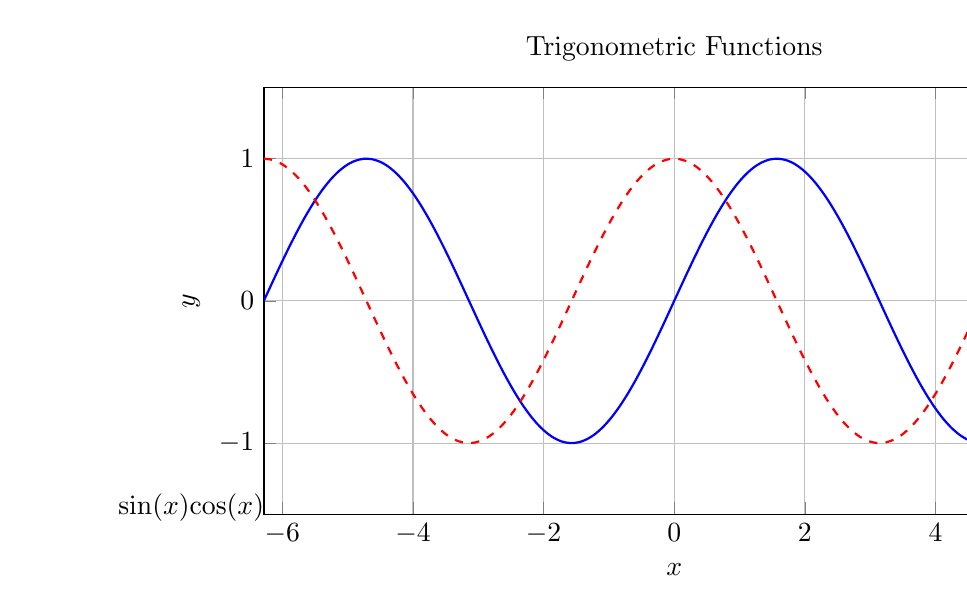
\begin{tikzpicture}
\begin{axis}[
    title={Trigonometric Functions},
    xlabel={$x$},
    ylabel={$y$},
    xmin=-6.28, xmax=6.28,
    ymin=-1.5, ymax=1.5,
    grid=major,
    legend pos=north east,
    width=12cm, height=7cm,
]
    \addplot[blue, thick, smooth, domain=-2*pi:2*pi, samples=100] {sin(deg(x))};
    \addlegend{$\sin(x)$}

    \addplot[red, thick, dashed, smooth, domain=-2*pi:2*pi, samples=100] {cos(deg(x))};
    \addlegend{$\cos(x)$}
\end{axis}
\end{tikzpicture}

\vspace{1cm}

% --- Bar chart ---
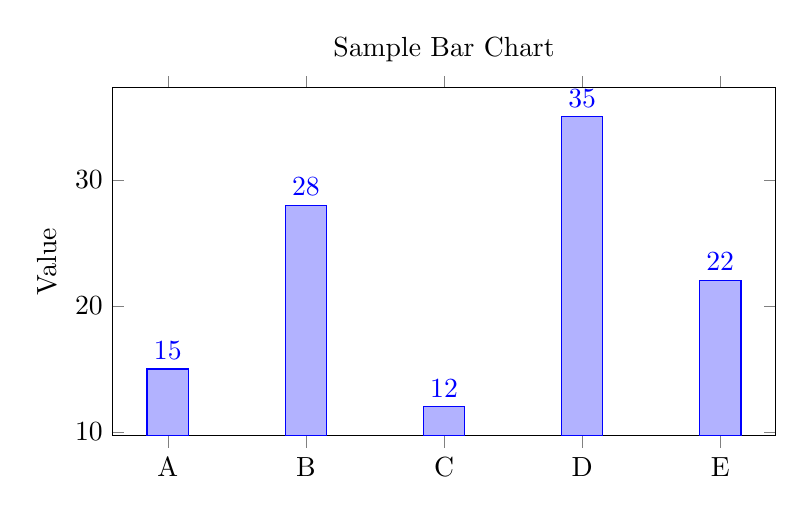
\begin{tikzpicture}
\begin{axis}[
    title={Sample Bar Chart},
    ybar,
    symbolic x coords={A, B, C, D, E},
    xtick=data,
    ylabel={Value},
    nodes near coords,
    width=10cm, height=6cm,
    bar width=15pt,
]
    \addplot coordinates {(A,15) (B,28) (C,12) (D,35) (E,22)};
\end{axis}
\end{tikzpicture}

\vspace{1cm}

% --- Scatter plot with data points ---
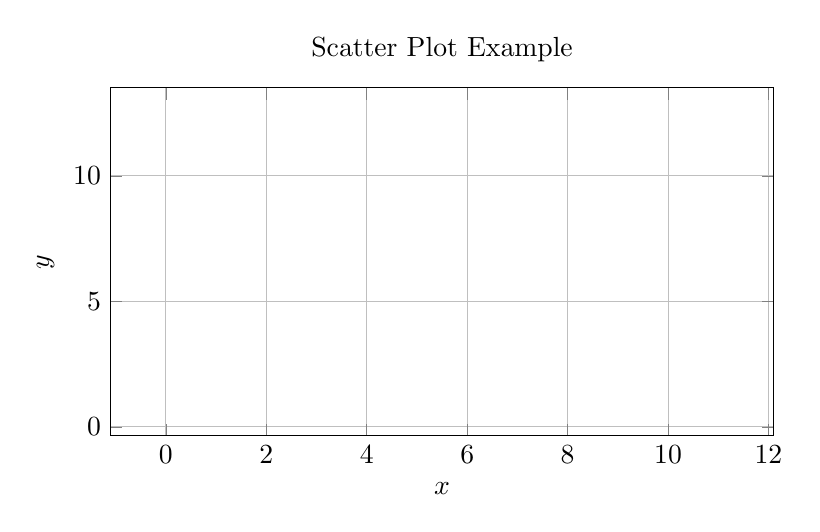
\begin{tikzpicture}
\begin{axis}[
    title={Scatter Plot Example},
    xlabel={$x$},
    ylabel={$y$},
    grid=both,
    width=10cm, height=6cm,
    only marks,
    mark=*,
    mark size=2pt,
]
    \addplot[blue] coordinates {
        (1,2) (2,3.5) (3,4) (4,5.2) (5,6.1)
        (6,7) (7,8.5) (8,9) (9,10.2) (10,11)
    };
    \addplot[red, domain=0:11, thick, no marks] {1.05*x + 0.8};
    \addlegend{Data points}
    \addlegend{Linear fit}
\end{axis}
\end{tikzpicture}

\end{document}
